\subsection{Convenção para fixar sistemas de coordenadas aos elos}
\label{sec:convencao_sistCoordenadas_elos}

Para descrever a localização de cada elo relativo ao seus elos vizinhos, foram fixados eixos em cada elo. Cada elo recebe o nome por um número de acordo com o elo que está sendo fixado, portanto o referencial $\{i\}$ é rigidamente fixado ao elo $\{i\}$.
Nesta pesquisa, a definição dos referenciais do manipulador de três juntas revolutas segue a convenção clássica de \gls{dh} para representar a transformação geométrica entre eles \cite{craig2005}, como mostrado na Figura~\ref{fig:Craig_3_5}.

\subsection{Convenção e descrição dos elos do manipulador robótico}
\label{sec:convencao_dh_mr}

Neste trabalho adota-se as convenções seguidas por \cite{craig2005}, adpatadas para aplicações espaciais.
Cada junta é associada a um eixo $\hat{Z}_i$, coincidente com o respectivo eixo de rotação.
O eixo $\hat{X}_i$ é orientado de modo a conectar o eixo $\hat{Z}_i$ ao eixo $\hat{Z}_{i+1}$, sendo perpendicular a ambos, enquanto $\hat{Y}_i$ é obtido pela regra da mão direita, completando o sistema ortogonal.
As juntas 1, 2 e 3 são revolutas, portanto os eixos $\hat{Z}_1$, $\hat{Z}_2$ e $\hat{Z}_3$ representam os eixos de rotação sucessivos dos elos.
O eixo $\hat{X}_1$ é definido na direção da interseção entre $\hat{Z}_1$ e $\hat{Z}_2$, e o eixo $\hat{X}_2$ segue o mesmo critério em relação a $\hat{Z}_2$ e $\hat{Z}_3$, a Figura~\ref{fig:Craig_3_5} demonstra isso. Por fim, o efetuador $\{E\}$ é definido na extremidade da ferramenta, que está rigidamente acoplada ao elo 3, de modo que o eixo $\hat{Z}_3$ permanece alinhado ao eixo longitudinal da ferramenta.
Os referenciais locais $\{i\}$ ($i=1,\dots,3$) fixados em cada elo do manipulador respeitam as convenções de \gls{dh}, e as distâncias e ângulos definidos a partir desses eixos são utilizados na construção da tabela \gls{dh}.


\begin{figure}[H]
\centering
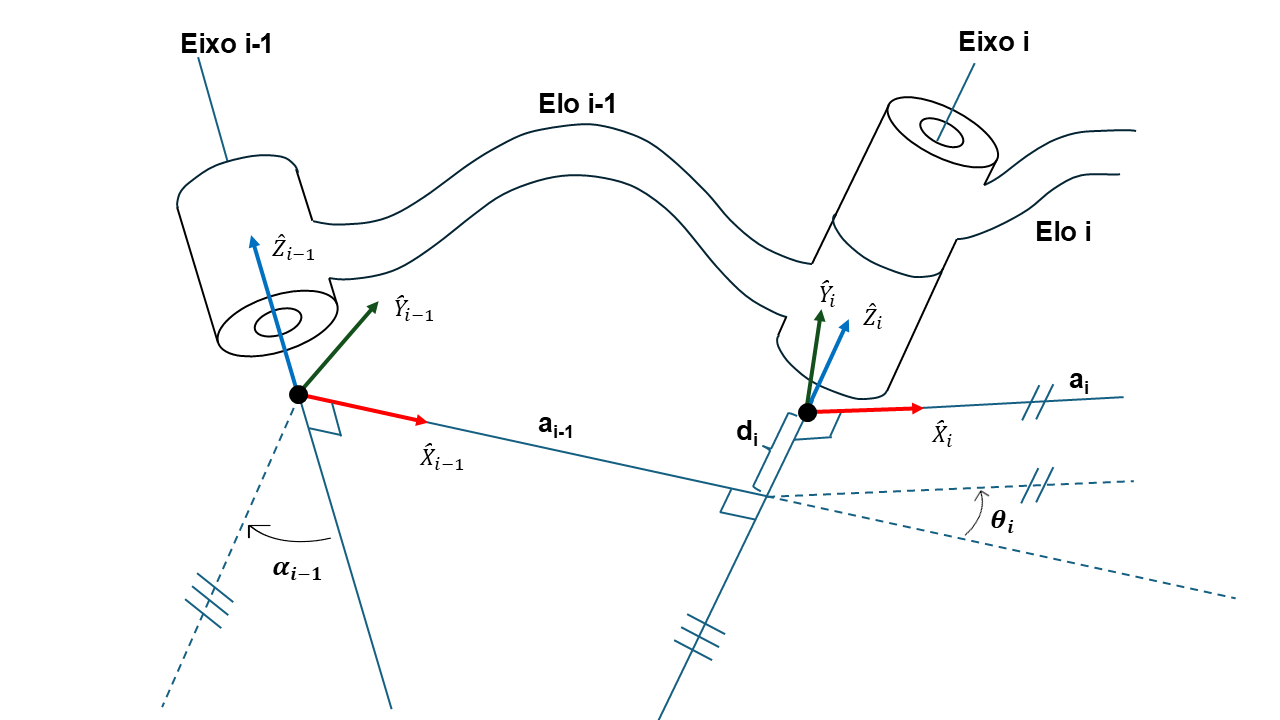
\includegraphics[width=0.9\textwidth]{3 Formulacao matematica/4 Manipulador robotico/Imagens_MR/Craig_3_5.png}
\caption{Referencias dos elos fixados de modo que o referencial $i$ é rigidamente fixado ao elo $i$. Adaptado de \cite{craig2005}.}
\label{fig:Craig_3_5}
\end{figure}

% Além da descrição geométrica, os mesmos referenciais e as transformações homogêneas sucessivas ${}^{B}T_i$ são reutilizados na formulação dinâmica do conjunto base--manipulador, sendo que a partir dessas matrizes obtêm-se as posições dos centros de massa e os eixos de junta em coordenadas da base, que são empregados no cálculo das matrizes de inércia espacial e dos Jacobianos espaciais. Esses elementos compõem o modelo de Lagrange implementado por meio de cadeias de transformações homogêneas sucessivas (rotações $R_Z$, $R_X$ e translações ao longo dos eixos globais), equivalentes à convenção de \gls{dh} adotada nesta seção.

A Figura~\ref{fig:referenciais_MR} exibe a espaçonave perseguidora de forma que é possível verificar os eixos de rotação de cada junta e o alinhamento de cada elo e os centros de gravidade de cada elemento.

\begin{figure}[ht]
\centering

\includegraphics[width=0.9\textwidth]{3 Formulacao matematica/4 Manipulador robotico/Imagens_MR/Lateral direita com eixos.png}
\caption{Referencial local do Manipulador Robótico 3R acoplado à base.}
\label{fig:referenciais_MR}
\end{figure}

Por sua vez, a Figura~\ref{fig:rotacaoJuntas_MR} exibe o mesmo manipulador robótico da Figura~\ref{fig:referenciais_MR}, no entanto, está no formato esquemático e explicita as juntas e seus eixos de rotação.
O sistema de coordenadas \gls{lvlh} é utilizado como referência no movimento relativo, enquanto o referencial da base $\{B\}$ é fixado na plataforma robótica da espaçonave e seus eixos estão alinhados conforme a orientação do corpo.
Neste trabalho é assumido que o referencial $\{0\}$ é tomado coincidente com a base física $\{B\}$, com $\hat{Z}_0$ alinhado ao eixo da primeira junta, de modo que as transformações homogêneas ${}^{B}T_i$ partem diretamente da base da primeira junta revoluta.

\begin{figure}[ht]
\centering

\includegraphics[width=0.9\textwidth]{3 Formulacao matematica/4 Manipulador robotico/Imagens_MR/Craig_3_6_RotacaoJuntas.png}
\caption{Notação esquemática do Manipulador Robótico 3R.}
\label{fig:rotacaoJuntas_MR}
\end{figure}

\subsubsection{Tabela de Denavit--Hartenberg}

Para dar continuidade com a modelagem matemática do \gls{mr}, a Tabela~\ref{tab:dh_zxx} foi construída seguindo a convenção de Denavit--Hartenberg apresentada em \cite{craig2005}. As variáveis presentes na tabela \gls{dh} são:

\begin{itemize}
    \item $a_i$: distância de $\hat{Z}_i$ até $\hat{Z}_{i+1}$ medida ao longo de $\hat{X}_i$;
    \item $\alpha_i$: ângulo de $\hat{Z}_i$ até $\hat{Z}_{i+1}$ medido em torno de $\hat{X}_i$;
    \item $d_i$: distância de $\hat{X}_{i-1}$ até $\hat{X}_i$ medida ao longo de $\hat{Z}_i$; e
    \item $\theta_i$: ângulo de $\hat{X}_{i-1}$ até $\hat{X}_i$ medido em torno de $\hat{Z}_i$.
\end{itemize}

O manipulador robótico possui três juntas revolutas, com eixos orientados segundo o arranjo $Z$--$X$--$X$: a junta~1 gira em torno de um eixo vertical $\hat{Z}$, enquanto as juntas~2 e~3 giram em torno de eixos paralelos ao eixo $\hat{X}$. Essa configuração estabelece diretamente a estrutura geométrica utilizada.

A definição dos parâmetros \gls{dh} decorre da orientação relativa entre os eixos de junta. Como a junta~1 gira em torno de um eixo vertical, $\hat{Z}_0$ e $\hat{Z}_1$ são coincidentes, o que implica $\alpha_0 = 0^\circ$ e $a_0 = 0$. Na junta~2, o eixo $\hat{Z}_2$ passa a ser orientado ao longo de $\hat{X}$, exigindo uma rotação de $90^\circ$ em torno de $\hat{X}_1$ para alinhar $\hat{Z}_1$ com $\hat{Z}_2$, resultando em $\alpha_1 = 90^\circ$. As juntas~2 e~3 possuem eixos paralelos, ambos orientados em $\hat{X}$, de modo que $\alpha_2 = 0^\circ$.

As juntas 2 e 3 são paralelas e implica que $a_2$, de $z_2$ para $z_3$ existe, e os termos $d_i$ são definidos como zero por não haver deslocamentos ao longo de $\hat{Z}_i$. As variáveis articulares $\theta_i$ correspondem diretamente às rotações das três juntas em torno de seus respectivos eixos $\hat{Z}_i$.

\begin{table}[ht]
\centering
\caption{Parâmetros DH do manipulador 3R Z--X--X (somente orientação)}
\label{tab:dh_zxx}
\begin{tabular}{c|c|c|c|c}
$i$ & $\alpha_{i-1}$ & $a_{i-1}$ & $d_i$ & $\theta_i$ \\
\hline
1 & $0^\circ$  & 0 & 0 & $\theta_1$ \\
2 & $90^\circ$ & 0 & 0 & $\theta_2$ \\
3 & $0^\circ$  & $a_2$ & 0 & $\theta_3$ \\
\end{tabular}
\end{table}

Dessa forma, a Tabela~\ref{tab:dh_zxx} resume a estrutura orientacional do \gls{mr} 3R $Z$--$X$--$X$, servindo de base para a formulação da cinemática direta de orientação e para a modelagem dinâmica subsequente.

\subsubsection{Transformações entre elos}
\label{sec:transformacoes_elos}

A transformação homogênea entre os referenciais consecutivos $\{i-1\}$ e $\{i\}$ é obtida a partir da convenção de \gls{dh} \cite{craig2005}.
Cada transformação representa a relação geométrica entre dois elos adjacentes e depende dos quatro parâmetros do elo $(\alpha_{i-1}, a_{i-1}, d_i, \theta_i)$.

A matriz de transformação $^{i-1}T_i$ é construída pela composição de quatro operações fundamentais: uma rotação de $\alpha_{i-1}$ em torno de $\hat{X}_{i-1}$, seguida de uma translação de $a_{i-1}$ ao longo de $\hat{X}_{i-1}$, uma rotação de $\theta_i$ em torno de $\hat{Z}_i$ e, por fim, uma translação de $d_i$ ao longo de $\hat{Z}_i$.
A forma geral da transformação é dada por \cite{craig2005}

\begin{equation}
    {}^{i-1}T_i
    =
    R_X(\alpha_{i-1})\,D_X(a_{i-1})\,R_Z(\theta_i)\,D_Z(d_i).
    \label{eq:Ti}
\end{equation}

As quatro matrizes da convenção de \gls{dh} são \cite{spong2006robot}:

\begin{equation}
R_X(\alpha_{i-1}) =
\begin{bmatrix}
1 & 0 & 0 & 0 \\
0 & \cos\alpha_{i-1} & -\sin\alpha_{i-1} & 0 \\
0 & \sin\alpha_{i-1} &  \cos\alpha_{i-1} & 0 \\
0 & 0 & 0 & 1
\end{bmatrix},
\end{equation}

\begin{equation}
D_X(a_{i-1}) =
\begin{bmatrix}
1 & 0 & 0 & a_{i-1} \\
0 & 1 & 0 & 0 \\
0 & 0 & 1 & 0 \\
0 & 0 & 0 & 1
\end{bmatrix},
\end{equation}

\begin{equation}
R_Z(\theta_i) =
\begin{bmatrix}
\cos\theta_i & -\sin\theta_i & 0 & 0 \\
\sin\theta_i &  \cos\theta_i & 0 & 0 \\
0 & 0 & 1 & 0 \\
0 & 0 & 0 & 1
\end{bmatrix},
\end{equation}

\begin{equation}
D_Z(d_i) =
\begin{bmatrix}
1 & 0 & 0 & 0 \\
0 & 1 & 0 & 0 \\
0 & 0 & 1 & d_i \\
0 & 0 & 0 & 1
\end{bmatrix}.
\end{equation}

Multiplicando essas quatro operações na ordem prescrita, conforme a equação \eqref{eq:Ti}, obtém-se a matriz homogênea completa \cite{craig2005}

\begin{equation}
    \label{eq:transf_homogenea_geral_Craig}
^{i-1}T_i =
\begin{bmatrix}
\cos\theta_i & -\sin\theta_i & 0 & a_{i-1} \\
\sin\theta_i\cos\alpha_{i-1} &
\cos\theta_i\cos\alpha_{i-1} &
-\sin\alpha_{i-1} &
-\sin\alpha_{i-1}d_i \\
\sin\theta_i\sin\alpha_{i-1} &
\cos\theta_i\sin\alpha_{i-1} &
\cos\alpha_{i-1} &
\cos\alpha_{i-1}d_i \\
0 & 0 & 0 & 1
\end{bmatrix}.
\end{equation}

As transformações homogêneas representam, em uma única matriz $4 \times 4$, tanto a orientação quanto a posição de um elo em relação ao anterior.
Cada matriz ${}^{i-1}T_i$ descreve a rotação e a translação do referencial $\{i\}$ em relação ao referencial $\{i-1\}$, constituindo a forma geral da transformação entre elos consecutivos de um manipulador.
Essa formulação é utilizada no cálculo direto da cinemática de posição e orientação do efetuador, permitindo expressar a pose final em função das variáveis articulares do manipulador.

\subsubsection{Espaço das juntas}

Neste trabalho, a lei de controle é implementada no espaço das juntas, pois o controlador PD atua diretamente sobre as variáveis articulares de posição e velocidade.
Essa abordagem elimina a necessidade de conversão para o espaço cartesiano e permite a aplicação direta dos torques de controle nas juntas, permitindo maior correspondência física entre as ações de controle e o movimento do manipulador \cite{craig2005}.